
\documentclass[border=10pt]{standalone}
%%%<
\usepackage{verbatim}
%%%>
\usepackage[utf8]{inputenc}
\usepackage{dtklogos}
\usepackage{tikz}
\usetikzlibrary{mindmap,shadows}
\usepackage[hidelinks,pdfencoding=auto]{hyperref}
% Information boxes
\newcommand*{\info}[4][16.3]{%
  \node [ annotation, #3, scale=0.65, text width = #1em,color=white,fill=none,inner sep = 2mm ] at (#2) {%
  \list{$\bullet$}{\topsep=0pt\itemsep=0pt\parsep=0pt
    \parskip=0pt\labelwidth=8pt\leftmargin=8pt
    \itemindent=0pt\labelsep=2pt}%
    #4
  \endlist
  };
}
\begin{document}
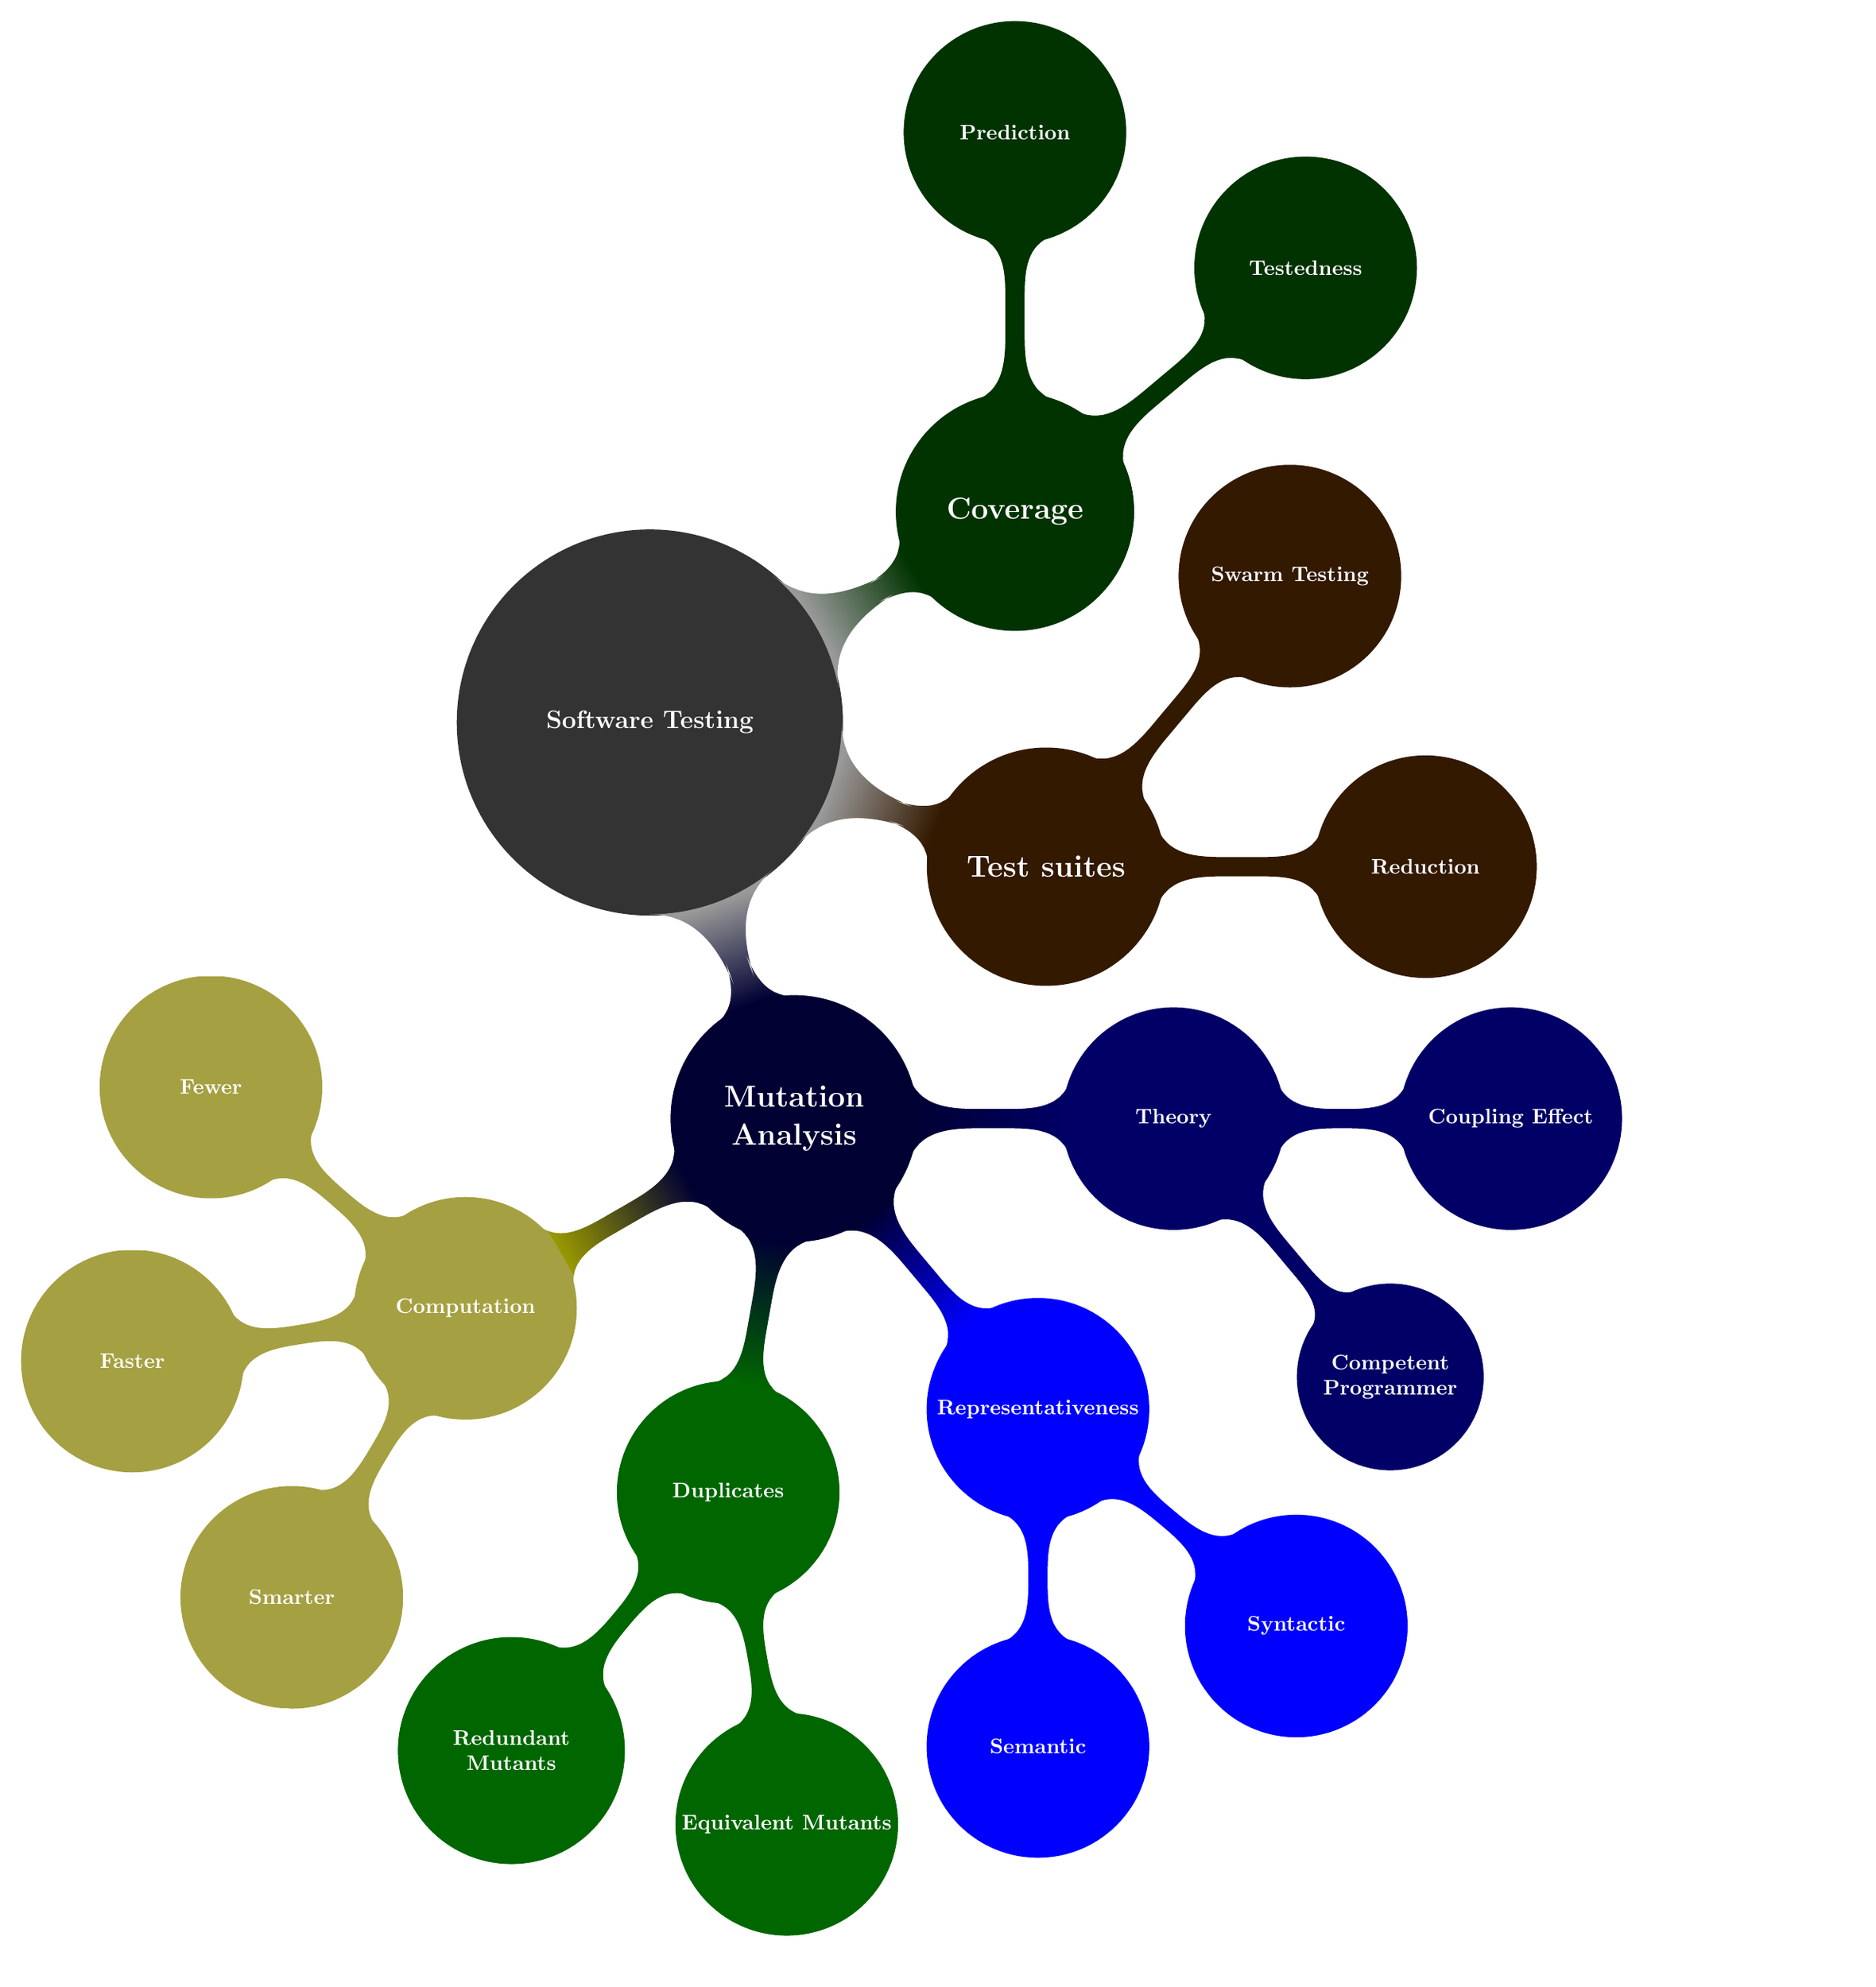
\begin{tikzpicture}[ every annotation/.style = {draw, fill = white, font = \Large}]
  \path[mindmap,concept color=black!40,text=white,
    every node/.style={concept},
    root/.style    = {concept color=black!80,font=\large\bfseries,text width=18em},
    level 1 concept/.append style={font=\Large\bfseries,sibling angle=50,text width=10.7em,level distance=20em,inner sep=2pt},
    level 2 concept/.append style={font=\bfseries,sibling angle=50,level distance=18em, text width=10em},
    level 3 concept/.append style={font=\bfseries,sibling angle=50,level distance=16em, text width=10em},
  ]
  node[root] {Software Testing} [clockwise from=30]
    child[concept color=green!20!black] {
      node[concept] {Coverage} [clockwise from=90]
    	child[concept color=green!20!black] { node (predictionN) {Prediction} }
    	child[concept color=green!20!black] { node (testednessN) {Testedness} }
    }
    child[concept color=orange!20!black] {
      node[concept] {Test suites} [clockwise from=50]
    	child[concept color=orange!20!black] { node (swarmN) {Swarm Testing} }
    	child[concept color=orange!20!black] { node (reductionN) {Reduction} }
    }
    child[concept color=blue!20!black] {
      node[concept] {Mutation Analysis} [clockwise from=0]
    	child[concept color=blue!40!black] {
          node {Theory} [clockwise from=0]
        	child { node (couplingN) {Coupling Effect} }
        	child { node [scale=1,text width=8em] (competentN) {Competent Programmer}  }
      }
      child[concept color=blue] {
        node[concept] {Representativeness} [clockwise from=320]
        child { node[concept] (syntacticN) {Syntactic} }
        child { node[concept] (semanticN) {Semantic} }
      }
      child[concept color=green!40!black] {
        node[concept] {Duplicates} [clockwise from=280]
        child { node[concept] (equivalentsN) {Equivalent Mutants} }
        child { node[concept] (redundantN) {Redundant Mutants} }
      }
      child[concept color=yellow!60!black] {
        node[concept] (Computation) {Computation} [clockwise from=239]
        child { node[concept] (smarterN) {Smarter} }
        child { node[concept] (fasterN) {Faster} }
        child { node[concept] (fewerN) {Fewer} }
      }
    };
    \info{swarmN.north east}{above,anchor=west,xshift=1em}{%
      \item 2016 ISSTA
    }
    \info{reductionN.north east}{above,anchor=west,xshift=1em}{%
      \item 2016 ASE
    }
    \info{predictionN.north east}{above,anchor=west,xshift=1em}{%
      \item 2014 ICSE
    }
    \info{testednessN.north east}{above,anchor=west,xshift=1em}{%
      \item 2016 FSE
    }
    \info{couplingN.north east}{above,anchor=west,xshift=1em}{%
      \item 2014 ISSRE
    }
    \info{competentN.south}{below,anchor=west,xshift=4em,yshift=2em}{%
      \item 2015 ISSRE
    }
    \info[9]{equivalentsN.south}{below,anchor=west,xshift=3em,yshift=-0.5em}{%
      \item 2015 ISSRE
    }
    \info[15]{redundantN.south}{below,anchor=west,xshift=-3em,yshift=-2em}{%
      \item 2016~Mutation
    }
    \info[14]{syntacticN.east}{anchor=west,xshift = 0.5em}{%
      \item 2014 ISSRE
    }
    \info[8]{smarterN.east}{anchor=north,xshift = -8em,yshift=-5em}{%
      \item 2016 ICSE
    }
    \info[10]{fasterN.east}{anchor=south,xshift = -6em,yshift=5em}{%
      \item 2016 ICSE
    }
    \info[14]{fewerN.east}{anchor=south,xshift = -5em,yshift=5em}{%
      \item 2016 ICSE
    }
\end{tikzpicture}
\end{document}
